\chapter[Metodologia]{Metodologia}
Neste capítulo é apresentado como foi realizada a implementação do algoritmo de treinamento do classificador LDA em um sistema coprocessado hardware-software, detalhando todos os módulos que compõem a implementação.

\section{Algoritmo Implementado}
Em 2010 o francês Fabien Lotte publicou um trabalho com objetivo de comparar as implementações de algoritmos de extração de características de sinais provenientes de atividades cerebrais, além de propor um novo algoritmo para extração de características dos sinais \cite{F.Lotte}.\\
Para coleta de resultados de seu trabalho, Lotte utilizou o algoritmo de classificação LDA e a base de dados \textit{BCI Competition III - Dataset IVa}, obtendo como melhor resultado o extrator de características CSP, conforme apresentado anteriormente na Tabela \ref{arte_state}.\\
O algoritmo foi desenvolvido utilizando a plataforma \textit{Matlab}, utilizando-se dos recursos e funções da plataforma. A Fig. \ref{processos_alg} apresenta um diagrama de atividades que descreve as funções utilizadas no algoritmo.

\begin{figure}[h]
	\centering
	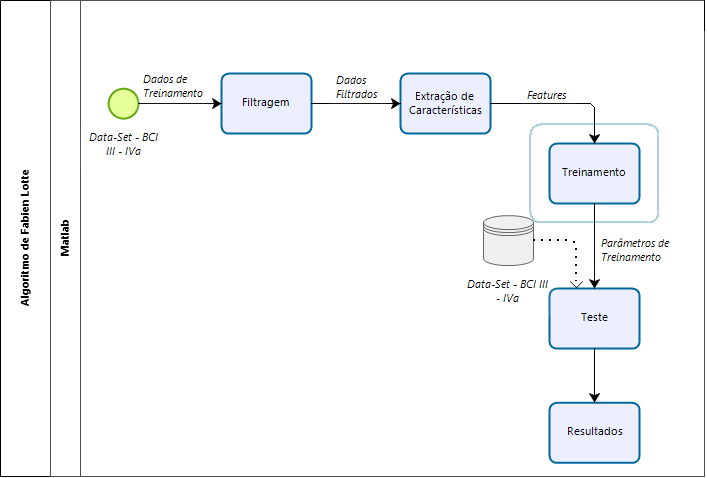
\includegraphics[keepaspectratio=true,scale=0.6]{figuras/Processos_Algoritmo_Lotte.PNG}
	\caption{Atividades realizadas pelo algoritmo de \cite{F.Lotte}.}
	\label{processos_alg}
\end{figure}

Utilizando-se dos dados de treinamento do \textit{BCI Competition III - Data Set -IVa}, o algoritmo inicia-se realizando a filtragem dos sinais a partir de um filtro \textit{Butterworth} passa faixas de {$5^a$} ordem, mantendo os sinais das faixas {$\alpha$} e {$\beta$} e atenuando as demais frequências. Em seguida, é realizado o processo de extração de características utilizando o algoritmo CSP. Logo após, é realizado o processo de treinamento, nos quais são calculados hiperplanos que melhor separam as classes. Estes hiperplanos são os parâmetros utilizados no processo de classificação, sendo então, um dos parâmetros de entrada da função de teste, nos quais são classificados os sinais de testes, também fornecidos pelo \textit{BCI Competition III - Data Set -IVa}. Por fim, são disponibilizados os resultados de acurácia e tempo de treinamento.

\section{Implementação em Sistema Coprocessado}

Conforme apresentado, o objetivo deste trabalho é o estudo dos ganhos ou perdas no processamento do algoritmo de treinamento do classificador LDA implementado em um coprocessamento hardware-software, utilizando-se do SoC \textit{Zynq} embarcado no kit de desenvolvimento \textit{Xilinx Zybo Board} modelo 70-10, comparado com a implementação realizada por \cite{F.Lotte} e a implementação em software executado sobre um SO Linux embarcado nos processadores ARM, também disponíveis no SoC. \\
Sendo assim, o trabalho se restringiu à implementação das atividades que compõem a função de treinamento do classificador LDA (atividades destacadas) na Fig. \ref{processos_alg}, em um sistema coprocessado .\\
A Fig. \ref{processos_train} apresenta um diagrama de atividades que descreve a função de treinamento do classificador LDA.

\begin{figure}[h]
	\centering
	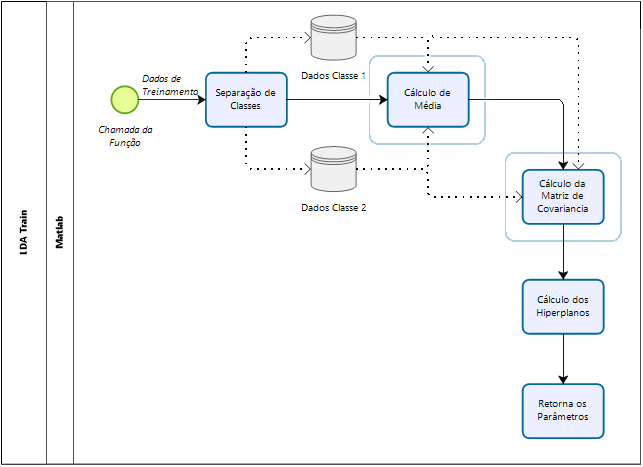
\includegraphics[keepaspectratio=true,scale=0.6]{figuras/Processos_LDA_Train.PNG}
	\caption{Atividades realizadas pelo algoritmo de treinamento do classificador LDA, desenvolvido por \cite{F.Lotte}.}
	\label{processos_train}
\end{figure}

Inicialmente é realizada a separação dos sinais em dois conjuntos de dados que representam os dados referentes às duas classes em estudo. Em seguida são calculadas as médias dos sinais de cada classe. Estes valores são repassados para a função de cálculo da matriz de covariância (ou dispersão), nos quais são realizados cálculos matriciais conforme apresentado na Equação \ref{eq: dispersaosb}. Posteriormente são calculados os hiperplanos a partir da covariância das características dos sinais. Estes hiperplanos representam os parâmetros de treinamento do classificador. São a partir deles que os sinais de teste são classificados.\\

Como será detalhado no capítulo seguinte as funções de cálculo de média e cálculo de covariância são as duas funções que apresentam um maior esforço computacional. Portanto ambas as funções foram mapeadas em hardware (funções destacadas na cor verde na Fig. \ref{processos_train}), utilizando-se da linguagem VHDL, a fim de acelerar o algoritmo de treinamento explorando o paralelismo dos algoritmos, enquanto as demais funções foram compiladas em software na linguagem C, executada através de um SO Linux embarcado nos processadores do SoC utilizado neste projeto.

\subsection{Ferramentas Utilizadas}
Para estudo das implementações foram utilizadas cinco ferramentas principais:\\
\begin{itemize}
	\item Software\textit{Matlab R2016a - \textit{Student License}} - Utilizado para reproduzir os resultados obtidos por \cite{F.Lotte};
	\item SO Linux - Utilizado como ambiente de desenvolvimento de software embarcado;
	\item Software \textit{Vivado - v.2017.4} - Utilizado para desenvolver, integrar e sintetizar os IP's de cálculo em ponto flutuante das funções média e covariância;
	\item \textit{Software Development Kit (SDK) - v.2017.4} - Utilizado para desenvolver o arquivo fsbl.elf e para compilar o arquivo BOOT.bin.
\end{itemize}

Para implementação em software e implementação coprocessada utilizamos o SoC \textit{Zynq} embarcado no kit de desenvolvimento \textit{Zybo Board}.

\subsection{Metodologias de Desenvolvimento}
\subsubsection{Implementação em Hardware}
Para implementação das funções de cálculo de média e cálculo da matriz de covariância em FPGA foi adotada a metodologia \textit{bottom-up}, na qual cada sub-bloco desenvolvido foi testado antes de ser inserido ao bloco principal, também conhecido como \textit{Top module}.
Os cálculos foram realizados através dos blocos de propriedade intelectual (IP) desenvolvidos por \cite{munoz2010tradeoff}. Os IPs realizam cálculos matemáticos em unidades de ponto flutuante de acordo com o padrão IEEE-754 \cite{IEEE745} com registradores de 27 bits, representados com:
\begin{itemize}
	\item Expoente: 8 bits;
	\item Mantissa: 18 bits;
	\item Sinal: 1 bit.
\end{itemize}

O IP que realiza o operação de soma ou subtração é controlado por uma máquina de estado finita (FSM - do inglês \textit{Finite State Machine}) \cite{munoz2010tradeoff}. O bloco apresentado na Fig. \ref{somador_27} representa o IP somador/subtrator, com suas respectivas entradas e saídas.

\begin{figure}[h]
	\centering
	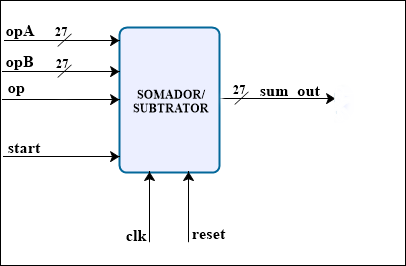
\includegraphics[keepaspectratio=true,scale=1]{figuras/bloco_soma.PNG}
	\caption{Representação do módulo somador/subtrator}
	\label{somador_27}
\end{figure}

O sinal de entrada oP representa se a função do bloco será soma (caso valor lógico for igual a 0) ou subtração (caso valor lógico for igual a 1) \cite{munoz2010tradeoff}. Os sinais opA e opB representam os valores de entrada, no caso da adição representam os valores da soma, e no caso da adição representam minuendo e subtraendo, respectivamente. Há também a entrada start utilizado para iniciar a operação assim que seu nível lógico realiza uma transição de borda de subida (de nível lógico 0 para nível lógico 1), além das entradas de clock e reset. 

Foram criados componentes para paralelizar o processo dos cálculos, buscando o maior nível de paralelismo. A partir do bloco de IP da Fig. \ref{somador_27}, para a função média foram implementados um total de 20 (vinte) somas em paralelo. Para sequenciar a soma final dos 20 operandos de entrada foi implementado um \textit{dataflow} de somadores, no qual a saída apresenta o resultado da soma final de 20 operandos (Fig. \ref{somador}). Já para a função de covariância foram implementados 4 componentes em paralelo que calculam parte da Equação \ref{eq: dispersaosb} conforme apresentado na Fig. \ref{covariancia}.

\begin{figure}[h]
	\centering
	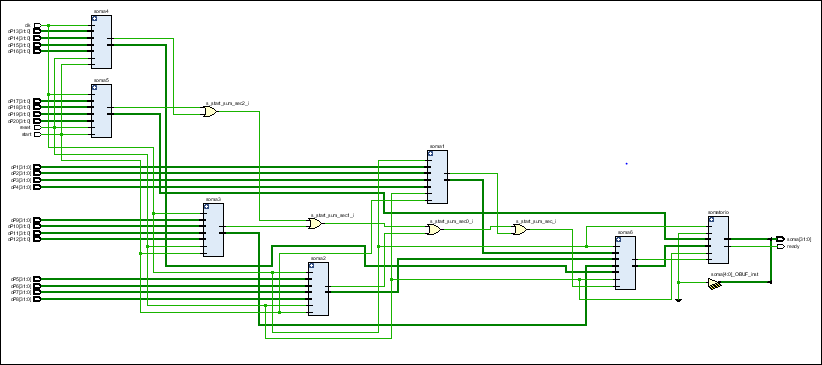
\includegraphics[keepaspectratio=true,scale=0.55]{figuras/rtl_media.png}
	\caption{Bloco para cálculo de média com vinte somas em paralelo.}
	\label{somador}
\end{figure}

Foram instanciados 5 blocos de somadores de 4 entradas, nomeados de soma primária, desenvolvidos a partir do bloco do IP somador da Fig. \ref{somador_27}. A saída de 4 (quatro) destes 5 (cinco) blocos são entradas de um novo bloco somador de 4 entrada, nomeado de soma secundária, com \textit{start} acionado após finalizar as somas primárias. A saída deste somador representa a entrada de um somador básico com 2 (duas) entradas, nomeado de soma final, completando a soma com a saída do $5^0$ (quinto) somador primário, resultando na saída final a soma dos 20 (vinte) operandos de entrada.
Após a soma de todos os valores pertencentes ao vetor de características de sua respectiva classe, o valor da soma total é dividido pela quantidade de sinais de características, resultando assim na média final de um determinado vetor de característica. 


A matriz de covariância é encontrada a partir de um cálculo matricial, conforme anteriormente apresentado na Equação \ref{eq: dispersaosb}. O cálculo implementado em hardware realiza o cálculo interno ao somatório, sendo então a Equação \ref{eq: cov_hw} implementada em hardware:

\begin{equation}
\label{eq: cov_hw}
cov_{hw} = \frac{(m_j - \bar m)(m_j -\bar m)}{n - 1} 
\end{equation}

A transposição da matriz (operator $^T$) e o somatório foi mantido em software. Sendo assim, o módulo apresenta 5 (cinco) saídas paralelas para cada uma das entradas da equação \ref{eq: cov_hw}.\\
\newpage

\begin{figure}[h]
	\centering
	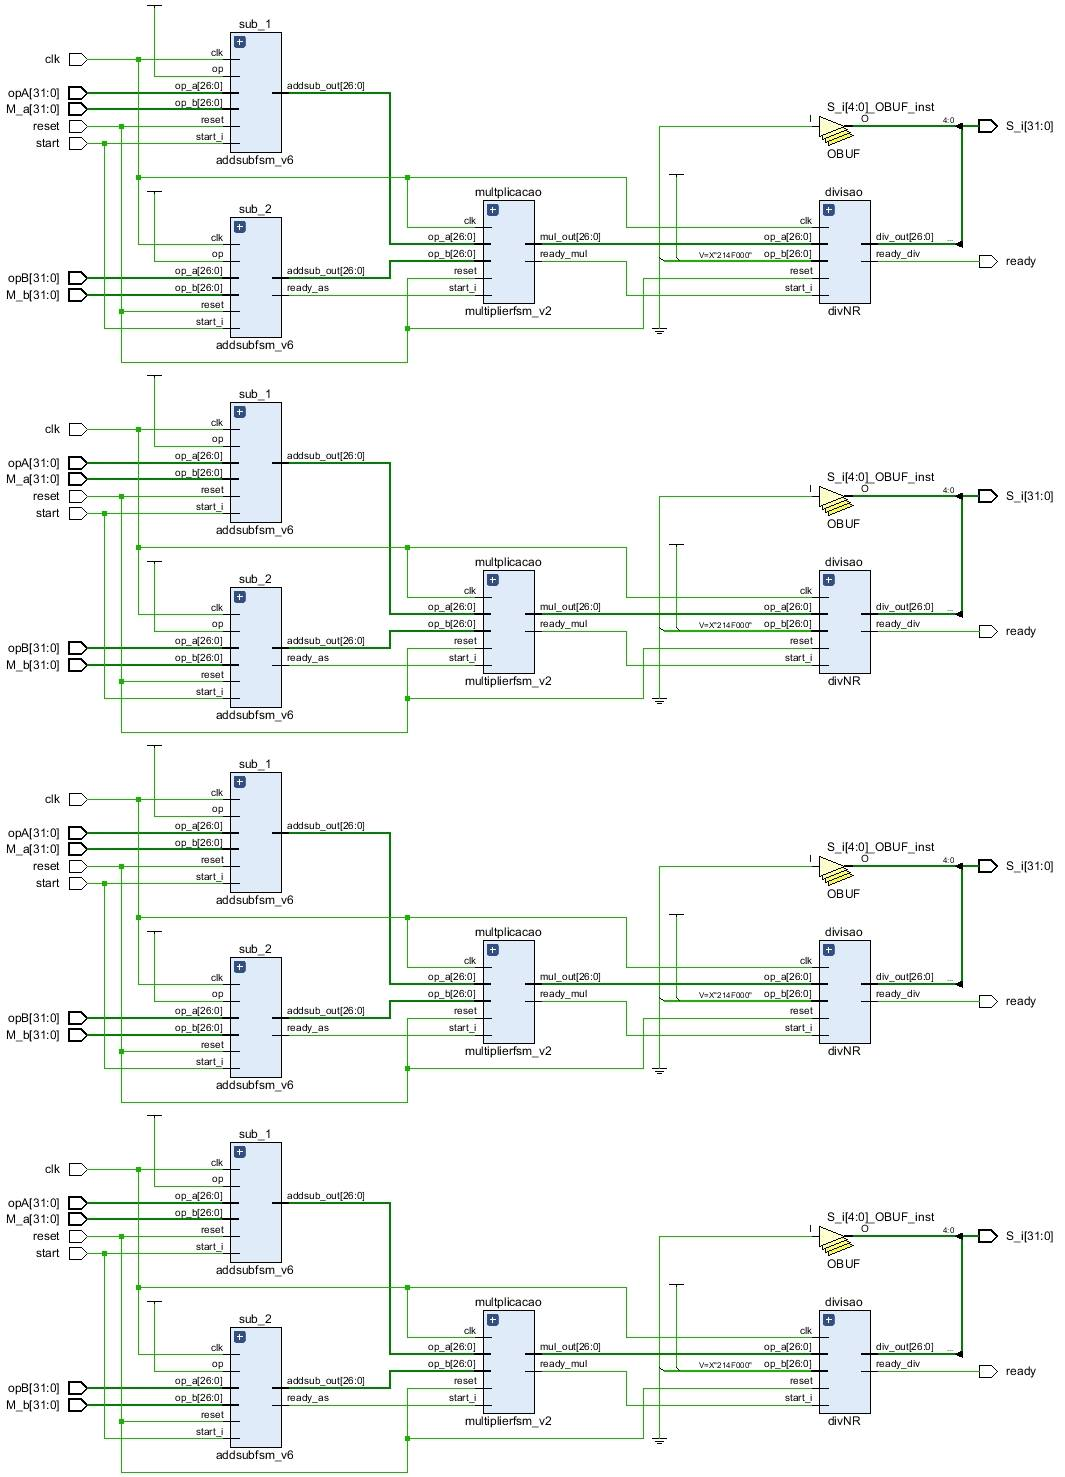
\includegraphics[keepaspectratio=true,scale=0.35]{figuras/rtl_covariancia.png}
	\caption{Bloco para cálculo da matriz de covariância com quatro cálculos em paralelo.}
	\label{covariancia}
\end{figure}

A técnica utilizada na implementação do projeto foi a \textit{dataflow}. O princípio básico das arquiteturas \textit{dataflow} é que a execução das operações é acionada em função da disponibilidade dos operandos. Ela não segue uma estrutura convencional de máquinas algorítmicas, no qual uma parte de controle é responsável pela sincronização das operações \cite{ThiagoUnB}. No caso dos sistemas em hardware implementados os blocos iniciam sua operação apenas quando suas entradas já estão carregadas.

Todos os módulos desenvolvidos foram atribuidos à um novo IP com barramento AXI4-Lite para realizar a comunicação com o procesador ARM. Nos quais são transmitido e recebido os dados de entrada referentes aos IPs de cálculo de média e cálculo da matrix de covariância. O diagrama geral da implementação, no qual é apresentado a conexão entre ARM e todos os seus periféricos, além dos IPs desenvolvidos é apresentado no ANEXO A deste trabalho.

O fluxo de desenvolvimento do projeto em hardware utilizado neste trablaho é apresentado na Fig. \ref{diagram_hardware}.

\begin{figure}[h]
  \centering
  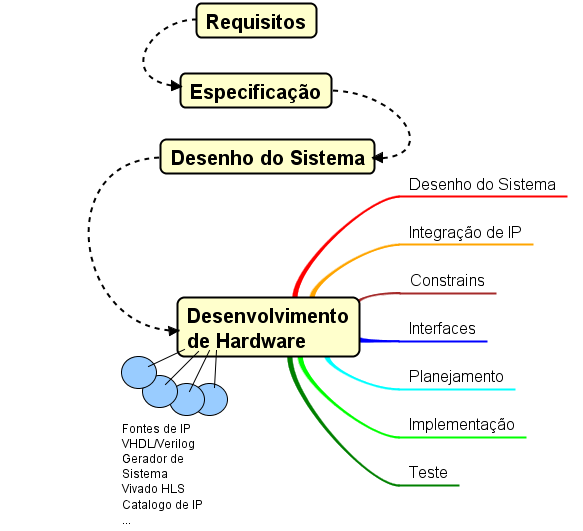
\includegraphics[keepaspectratio=true,scale=1.0]{figuras/fluxograma_hardware.PNG}
  \caption{Fluxograma de implementação de hardware em um SoC. Adaptado de \cite{zynqBook}}
  \label{diagram_hardware}
\end{figure}

\subsection{Protocolo Para Análise estatística}
Para efeito de análise estatística comparatória foram coletados as seguintes informações pós implementação:

\begin{itemize}[noitemsep]
	\item Consumo de hardware: LUTs, FFs, blocos de DSP, blocos de memória RAM, I/O;
	\item Dados de desempenho: frequência de operação e tempo de execução;
	\item Dados simulados: Latência e \textit{throughput};
	\item Estimação do consumo de energético;
	\item Estimação estatística do erro quadrático de implementação em hardware comparada com a implementação original em \textit{Matlab}.
\end{itemize}

\section{Implementação em software}

\subsection{Métodos e Técnicas}
Para o auxílio desta implementação, foi instalado o sistema operacional \textit{Debian Linux} sobre os cores ARM, cujos recursos e passos necessários
para a instalação do SO estão contidos no ANEXO B.

O processo para implementação seguiu o método \textit{bottom-up}, blocos de códigos menores foram implementados e testados separadamente, com a finalidade de todos os blocos serem integrados e testados em um único bloco principal. Todas as codificações foram implementadas utilizando a linguagem de programação C, e para compilar o código principal foi utilizado o compilador GCC \textit{(GNU Compiler Collection)}. Com esse método conseguimos realizar uma análise de perfil das funções implementadas reportando os tempo de execução de cada uma das funções, sendo assim possível deduzir as funções que necessitam de maior esforço computacional. As entradas para programa desenvolvido são os sinais de treinamento fornecidos pelo \textit{dataset IVa} do \textit{BCI Competition III}.

Como parâmetro de análise estatística foram coletados os seguintes dados:

\begin{itemize}[noitemsep]
\item Consumo de memória
\item Tempo de execução
\item Erro da implementação em comparação aos resultados obtidos por \cite{F.Lotte}
\end{itemize}

\section{Integração}
Toda a integração do projeto coprocessado é possibilitado pelo uso do barramento \textit{AXI4-Lite}, que interliga a PL com a PS, 
um esquemático do processo de escrita e leitura nos IP através do barramento \textit{AXI4-Lite} pode ser observado na Fig. \ref{axi_bus}
\newpage

\begin{figure}[h]
	\centering
	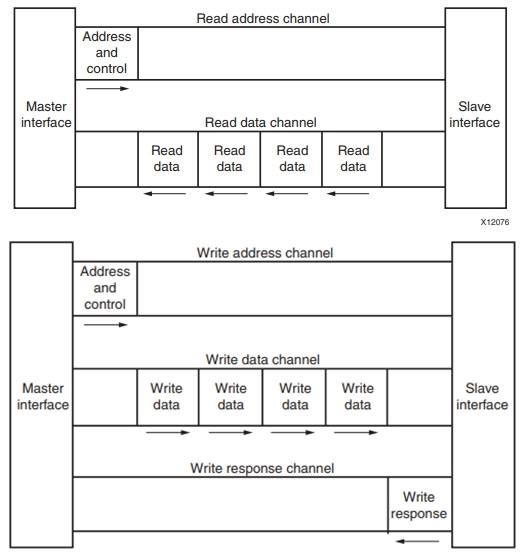
\includegraphics[keepaspectratio=true,scale=0.5]{figuras/axi_bus.png}
	\caption{Fluxo de dados para leitura e escrita no barramento AXI Fone: \cite{user-guide-axi}}
	\label{axi_bus}
\end{figure}

Para realizar escrita e leitura de dados nos IPs através da aplicação implementada em software, ultilizamos a função mmap() que faz parte da biblioteca <sys/mman.h>, esta função cria um novo mapeamento de memória no endereço de memória virtual no seu processo de chamada. Esse novo endereço começa no endereço de memória do IP (com AXI), com isso é possivel ler e escrever no endereço memória de de qualquer IP, desde que a memória esteja devidamente mapeada.

Como os IPs desenvolvidos por \cite{munoz2010tradeoff} realizam operações em ponto flutuante de 27 bits e o barramento \textit{AXI-4Lite} possui como configuração mínima de registradores o valor de 32 bits, em todos os IPs desenvolvidos as entradas e saídas possuem tamanho de 32 bits, porém para realização dos cálculo é considerada apenas os 27 bits mais significativos presentes nos registradores do barramento de comunicação \textit{AXI-4Lite}.
\vspace{\onelineskip}

